\chapter{Synthèse et optimisation des circuits séquentiels}
\section{Classes et représentation}
Rappelons que l'état du système n'est pas forcement visible par l'extérieur.\\
La sortie d'un système est fonction de l'état et \textit{éventuellement} des entrées. Cet \textit{éventuellement} implique 2 classes de circuit logique séquentiel:
\begin{itemize}
	\item Machine de Moore (pas Gordon!)
	\item Machine de Meally
\end{itemize}
\paragraph{Machine de Moore:}
la \textbf{sortie} est \textbf{uniquement} fonction des \textbf{variables d'état}.
\begin{figure}[H]
	\centering
	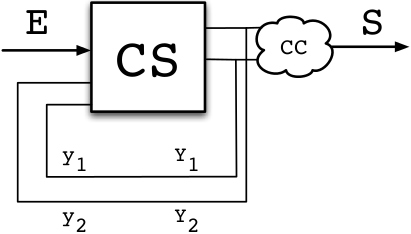
\includegraphics[width=.3\textwidth]{ch7/image1}
\end{figure}
\paragraph{Machine de Meally:}
la \textbf{sortie} est fonction (combinatoire) des \textbf{variables d'état} et des \textbf{entrées}.
\begin{figure}[H]
	\centering
	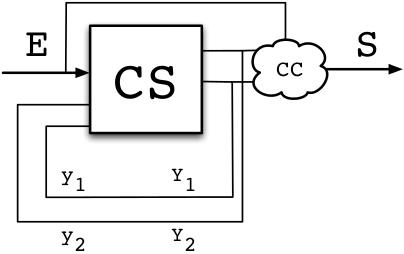
\includegraphics[width=.3\textwidth]{ch7/image2}
\end{figure}

Pour la synthèse à partir d'un cahier de charges verbal :
\begin{enumerate}
	\item Table d'état (ou Table de Huffman)
	\item Graphe d'état (optionnel)
	\item Équations logiques (et le circuit logique)
\end{enumerate}
\subsection{Codage des états}
On souhaite représenter les systèmes séquentiels à l'aide des codes binaires $\{0, 1, \text{-}\}$. Ce processus d'attribution de codes binaires aux états codés s'appelle \textit{le codage des états}.\\
Le nombre de bits nécessaires pour coder $n$ états est donné par $\log_2n$.
\subsubsection{Exemple}
Soit un système à 4 états. Attribuons à chaque état un code binaire (4 états $\rightarrow \log_2 4=2\rightarrow$ 2 bits nécessaires).\\
Ainsi $1\rightarrow 00,\ 2\rightarrow 01,\ 3\rightarrow 11,\ 4\rightarrow 10$.\\
Ainsi, on obtient:
\begin{figure}[H]
	\centering
	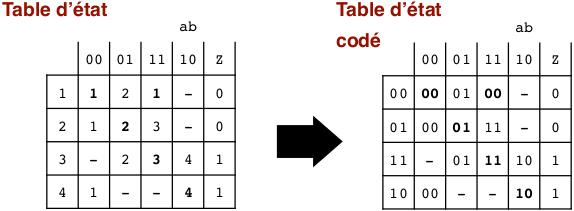
\includegraphics[width=.6\textwidth]{ch7/image3}
\end{figure}
À chaque bit du code correspond une fonction logique. On a donc : 4 états et 2 variables d'états ($y_2y_1$)$\rightarrow$ 2 fonctions logiques.
\begin{figure}[H]
	\centering
	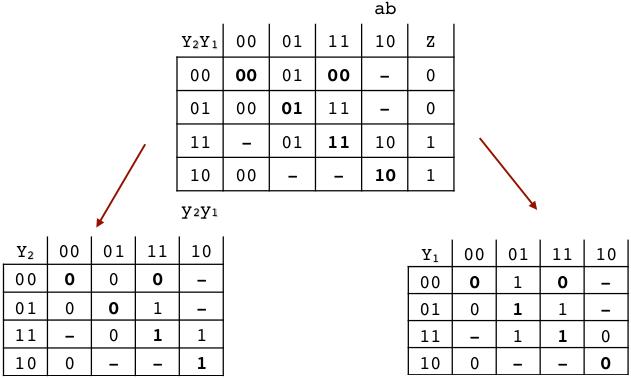
\includegraphics[width=.7\textwidth]{ch7/image4}
\end{figure}
Il suffit de simplifier la K-Map de $Y_2$ et celle de $Y_1$ et déduire leur fonction logique respective
\begin{figure}[H]
	\centering
	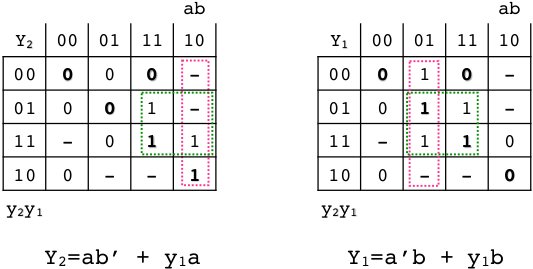
\includegraphics[width=.7\textwidth]{ch7/image5}
\end{figure}
\danger $y_2y_1\neq Y_2Y_1$, les premières représentent le présent, les 2 autres le futur.\\

Établissons la \textit{fonction de sortie}. Connaissant la valeur de sortie des états stables, nous pouvons remplir les cases correspondantes.
\begin{figure}[H]
	\centering
	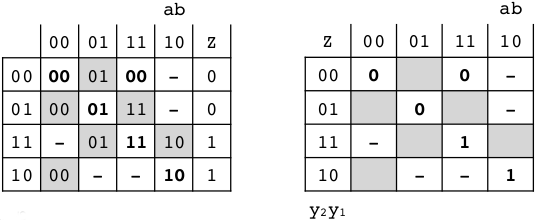
\includegraphics[width=.7\textwidth]{ch7/image6}
\end{figure} Pour les transitions (cases grises), il faut respecter les transitions ainsi que la règle suivante:
\begin{center}
	\textbf{Lors des transitions, si la sortie doit changer, elle ne devrait changer qu'une seule fois}
\end{center}
c-à-d que les \textbf{seules} possibilités sont
\begin{figure}[H]
	\centering
	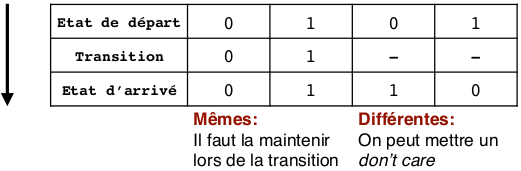
\includegraphics[width=.7\textwidth]{ch7/image7}
\end{figure}
Nous obtenons donc
\begin{figure}[H]
	\centering
	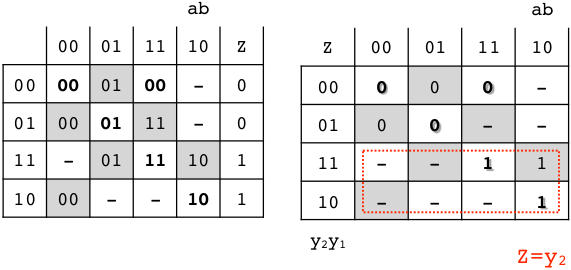
\includegraphics[width=.7\textwidth]{ch7/image8}
\end{figure}
Le logigramme correspondant n'est autre que
\begin{figure}[H]
	\centering
	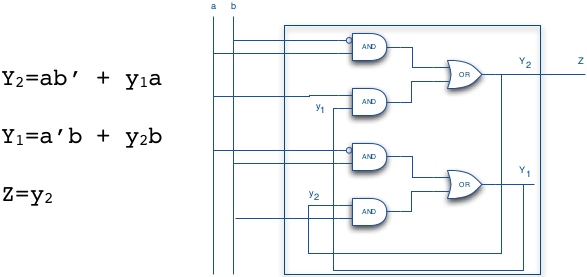
\includegraphics[width=.8\textwidth]{ch7/image9}
\end{figure}
\section{Simplification de la table primitive des états}
L’algorithme de synthèse se constitue de 3 étapes :
\begin{enumerate}
	\item Table primitive d'état ou Table de Huffman :
	\begin{itemize}
		\item Écrire la table de Huffman à partir d'un cahier de charges.
		\item La \textbf{1\up{ère}} table ne peut avoir qu'\textbf{un seul état stable par ligne de la table d'état}
	\end{itemize}
	\item Codage des états
	\item Équations logiques
\end{enumerate}
La complexité du circuit obtenu lors de la synthèse est influencé par la complexité (taille) de la taille initiale d'état.\\
Chaque bit de code ($\log_2n$ bits de code pour $n$ états) représente:
\begin{itemize}
	\item une fonction logique
	\item un organe de mémoire (délais)
\end{itemize}
Il faut donc réduire le nombre d'états pour simplifier le circuit correspondant.
\subsection{Réduction du nombre d'état}
\subsubsection{Notion d'équivalence de deux états}
Deux états sont équivalents si (équivalence de deux états stables):
\begin{enumerate}
	\item ils produisent la \textbf{même sortie}
	\item pour \textbf{toutes} combinaisons des variables d'entrée, les \textbf{futurs} états sont soit les mêmes soit \textbf{équivalents}
\end{enumerate}
Nous obtenons donc deux types d'équivalence:
\begin{itemize}
	\item \textbf{États identique} : 2 (ou plus) états stables sont au même endroit (même combinaison des entrées)
	\begin{figure}[H]
		\centering
		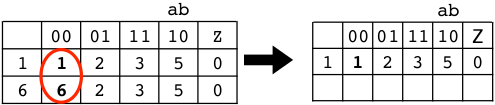
\includegraphics[width=.7\textwidth]{ch7/image10}
	\end{figure}
	\item \textbf{États fusionnables} : les états stables se trouvent à des endroits différents (combinaison des entrées différentes)
	\begin{figure}[H]
		\centering
		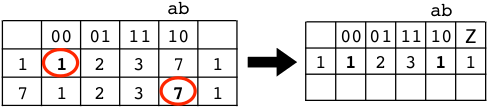
\includegraphics[width=.7\textwidth]{ch7/image11}
	\end{figure}
\end{itemize}
Pour que $n$-états soient équivalents il faut que tous les états soient équivalents deux à deux.\\

Pour ce faire, on dresse un tableau de $n(n-1)/2$ cases appelé \textbf{table des conditions d'équivalences}:
\begin{itemize}
	\item Chaque case de la table représente la possibilité d'équivalence et/ou de fusionnement de deux états
	\item \textbf{Dans le cas de la machine de Moore}, toute paire d'états ayant la sortie différente peut être exclue
	\item L'impossibilité de fusionner deux états se note par une croix
\end{itemize}
Pour 11 états, la table des conditions d'équivalence ressemble à:
\begin{figure}[H]
	\centering
	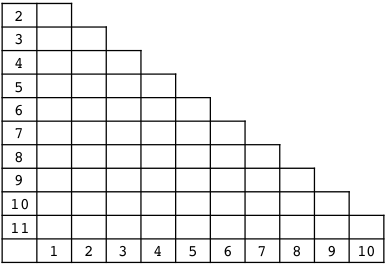
\includegraphics[width=.6\textwidth]{ch7/image12}
\end{figure}
\section{Synthèse d'un flip-flop D}
\begin{wrapfigure}{r}{.5\textwidth}
	\centering
	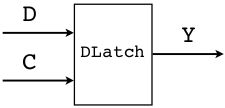
\includegraphics[width=.3\textwidth]{ch7/image13}
\end{wrapfigure}
\subsection{D-Latch:} Mémoire suiveuse-bloqueuse (\textit{Sample and Hold}).\\
Spécification:
\begin{itemize}
	\item 2 entrées : D (\textit{data}) et C (\textit{control})
	\item Une sortie : Y
	\item La sortie prend la valeur de l'entrée D lorsque C$=1$
\end{itemize}
\subsection{D Flip-Flop (\textit{edge triggered})}
\begin{wrapfigure}{r}{.5\textwidth}
	\centering
	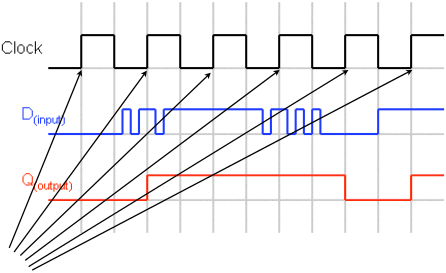
\includegraphics[width=.4\textwidth]{ch7/image14}
\end{wrapfigure}
Spécification :
\begin{itemize}
	\item La sortie prend la valeur de D \textbf{uniquement} lors d'un \textbf{flanc montant} de C (passage de $0\rightarrow 1$)
	\item Entre 2 flancs montants, la valeur de D est maintenue (toute variation de D est ignorée)
	\item Si C est sur un flanc montant et que D varie, la sortie prend l'ancienne valeur de D, celle juste avant le flanc montant 
	\item Le reste n'est que maintient
\end{itemize}
\subsubsection{Table primitive d'état}
\begin{minipage}{.5\textwidth}
	Considérons l'évolution qui mettra la sortie à 1:
\begin{enumerate}
	\item Situation de départ $\rightarrow Q=0$ et aucun changement à l'entrée (le $CD=00$ ne change pas) $\Rightarrow$ état 1
	\item $D$ change ($0\rightarrow 1$) avant $C$ $\Rightarrow$ état 2
	\item $C$ change $\Rightarrow$ état 4
\end{enumerate}
\end{minipage}
\vspace{-2.9cm}
\begin{minipage}{.5\textwidth}
	\begin{figure}[H]
		\centering
		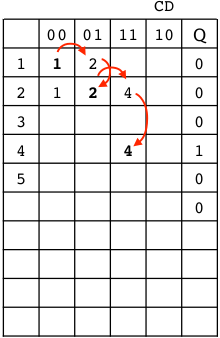
\includegraphics[width=.7\textwidth]{ch7/image15}
	\end{figure}
\end{minipage}
\begin{minipage}{.5\textwidth}
	Considérons maintenant une autre évolution en partant de l'état 1
	\begin{enumerate}
		\item $C$ change avant $D$ ($CD=00\rightarrow 10$) $\Rightarrow$ état 3
		\item $D$ change, le système ignore sa variation $\Rightarrow$ état 5 (diffère de l'état 4 par la valeur de la sortie $Q$)
	\end{enumerate}
\end{minipage}
\begin{minipage}{.5\textwidth}
	\begin{figure}[H]
		\centering
		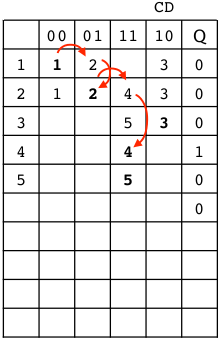
\includegraphics[width=.7\textwidth]{ch7/image16}
	\end{figure}
\end{minipage}

\begin{minipage}{.5\textwidth}
	Principe de mémorisation d'un 1
	\begin{enumerate}
		\item Initialement : $CD=00$
		\item $CD=00\rightarrow 01\rightarrow 11$
		\item $Q=0\rightarrow 1$ (état 4)
		\item $C=0 \Rightarrow$ peu importe la valeur de $D$, la sortie reste à 1 (états 7 et 9)
	\end{enumerate}
\end{minipage}
\begin{minipage}{.5\textwidth}
	\begin{figure}[H]
		\centering
		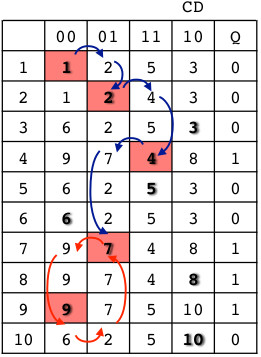
\includegraphics[width=.7\textwidth]{ch7/image17}
	\end{figure}
\end{minipage}

\subsubsection{Table de conditions d'équivalences}
Cette table se définit en 3 passes:
\begin{enumerate}
	\item[-- Passe 1.] Sorties différentes
	\begin{figure}[H]
		\centering
		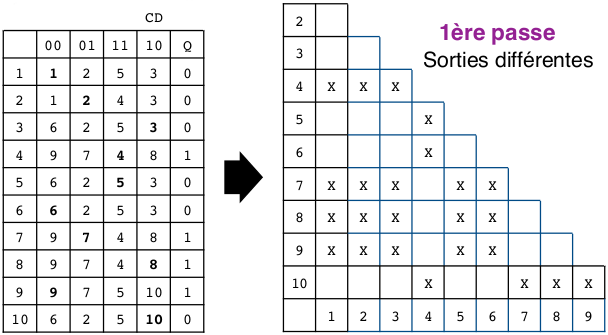
\includegraphics[width=.7\textwidth]{ch7/image18}
	\end{figure}
	\item[-- Passe 2.] Conditions de fusionnements 
	\begin{figure}[H]
		\centering
		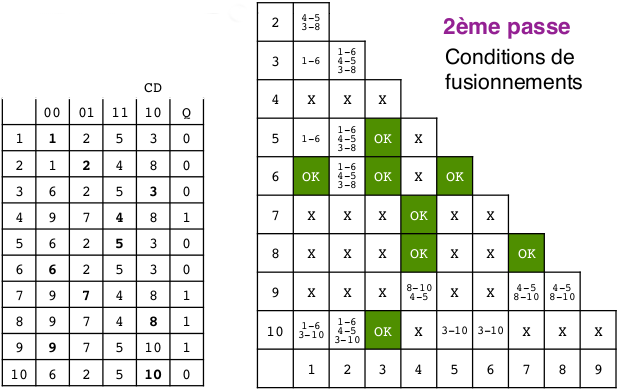
\includegraphics[width=.7\textwidth]{ch7/image19}
	\end{figure}
	\item[-- Passe 3.] Suppression des impossibles
	\begin{figure}[H]
		\centering
		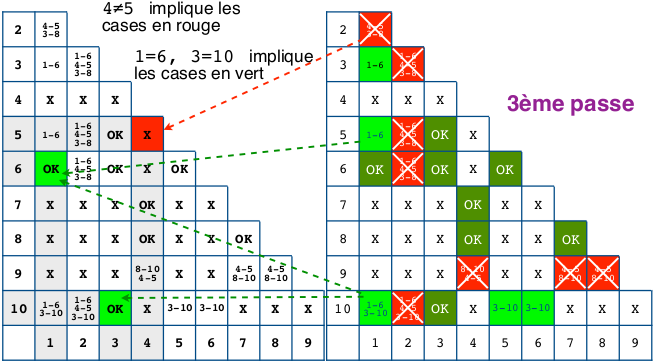
\includegraphics[width=.7\textwidth]{ch7/image20}
	\end{figure}
\end{enumerate}
Nous pouvons donc obtenir de ce tableau une liste assez claire des fusionnements possibles :
\begin{figure}[H]
	\centering
	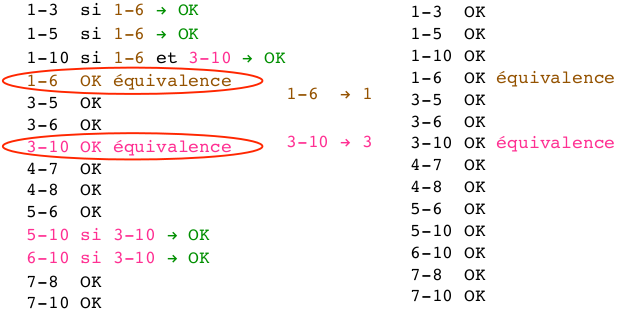
\includegraphics[width=.7\textwidth]{ch7/image21}
\end{figure}
Après avoir établi nos choix de fusionnement, il suffit de les appliquer à la table primitive d'état et de réordonner pour plus de lisibilité :
\begin{figure}[H]
	\centering
	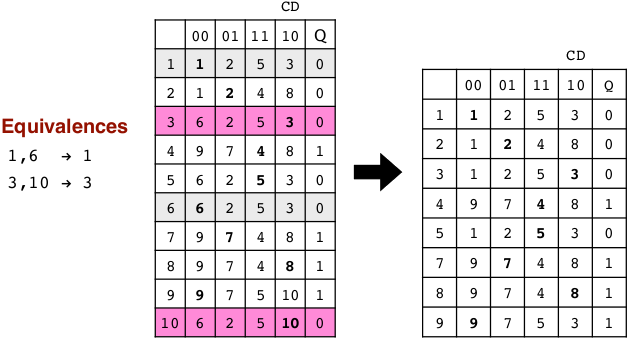
\includegraphics[width=.7\textwidth]{ch7/image22}
\end{figure}
Nous passons donc de 10 à 4 états $\Rightarrow$ 2 variables d'état au lieu de 4 !\\

Le choix du codage des états étant (pour l'instant) arbitraire : $1\rightarrow 00,\ 2\rightarrow 01,\ 3\rightarrow 11,\ 4\rightarrow 10$. Il ne reste plus qu'à écrire la K-Map de chaque variable d'état et d'en déduire leur fonction logique:
 \begin{figure}[H]
 	\centering
 	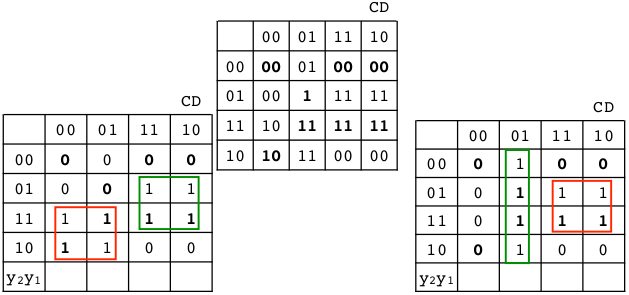
\includegraphics[width=.7\textwidth]{ch7/image23}
 \end{figure}
\section{Différents organes de mémoire}
Nous verrons 4 type de flip-flop :
\begin{itemize}
	\item SR : $Q=1$ lorsque $S=1$. La combinaison $SR=11$ est interdite.
	\item JK : même chose que SR mais la combinaison interdite change d'état
	\item D : la sortie suit l'entrée
	\item T : changement d'état lorsque l'entrée $T=1$
\end{itemize}
\subsection{Description des flip-flops}
Nous verrons 3 manières pour décrire un flip-flop :
\begin{itemize}
	\item Table de fonctionnement (sorte de table d'état)
	\item Équations caractéristiques
	\item Table d'excitation 
\end{itemize}
On notera l'état présent par un Q et l'état futur par un Q\up{+}. À cela s'ajoute (pour la table d'excitation) 4 possibilités de couple présent-futur
\begin{figure}[H]
	\centering
	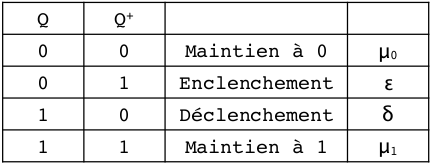
\includegraphics[width=.5\textwidth]{ch7/image24}
\end{figure}
\subsubsection{Flip-flop SR}
\begin{figure}[H]
	\centering
	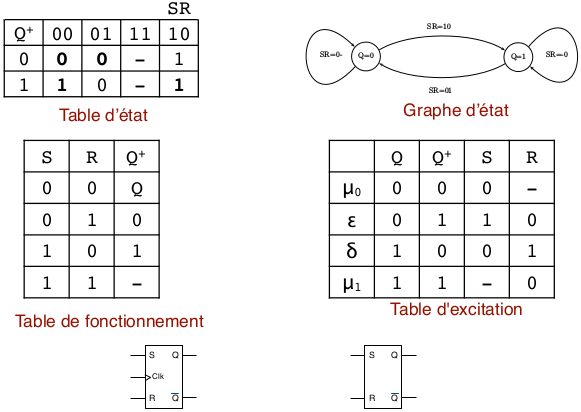
\includegraphics[width=.8\textwidth]{ch7/image25}
	\caption{Représentation schématique flip-flop SR}
\end{figure}
\subsubsection{Flip-flop JK}
\begin{figure}[H]
	\centering
	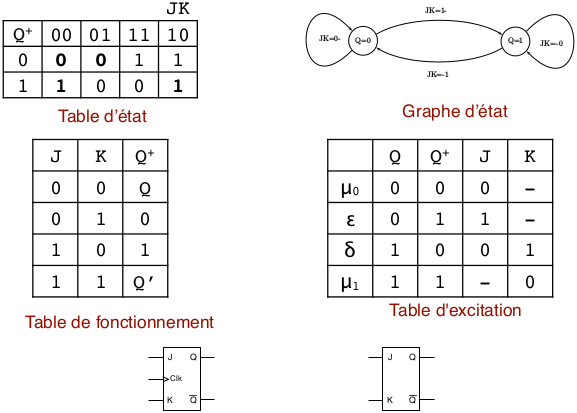
\includegraphics[width=.8\textwidth]{ch7/image26}
	\caption{Représentation schématique flip-flop JK}
\end{figure}
\subsubsection{Flip-flop D}
\begin{figure}[H]
	\centering
	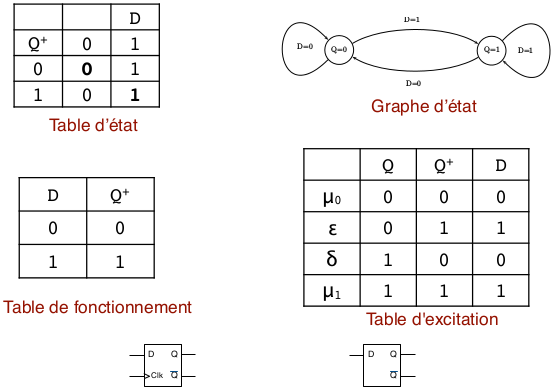
\includegraphics[width=.8\textwidth]{ch7/image27}
	\caption{Représentation schématique flip-flop D}
\end{figure}
\subsubsection{Flip-flop T}
\begin{figure}[H]
	\centering
	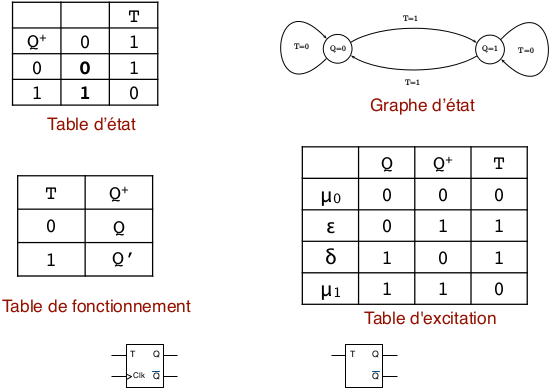
\includegraphics[width=.8\textwidth]{ch7/image28}
	\caption{Représentation schématique flip-flop T}
\end{figure}
\section{Courses critiques}
L'un des problèmes fondamental des circuits réels logiques à rétroaction est le problème des courses critiques. Il existe 2 méthodes de résolution des courses critiques 
\begin{itemize}
	\item Action sur le \textbf{codage des états} et les transitions $\Rightarrow$ conception des systèmes \textbf{séquentiels asynchrones}
	\item Action sur la \textbf{mise à jour} des variables d'état $\Rightarrow$ conception des systèmes \textbf{séquentiels synchrones}
\end{itemize}
\subsection{Origine du problème des courses critiques}
Prenons une table d'état déjà codée et faisons l'hypothèse que nous sommes dans l'état $00$ stable (c-à-d $ab=00$). Changeons les valeurs d'entrée $ab=00\rightarrow 11$. D'après la table, nous devons aller à l'état $11$. Nous avons donc $Y_1Y_2=00\rightarrow 11$. Regardons ce qu'il se passe en pratique
\begin{figure}[H]
	\centering
	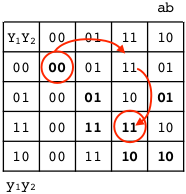
\includegraphics[width=.3\textwidth]{ch7/image29}
\end{figure}
\begin{figure}[H]
	\centering
	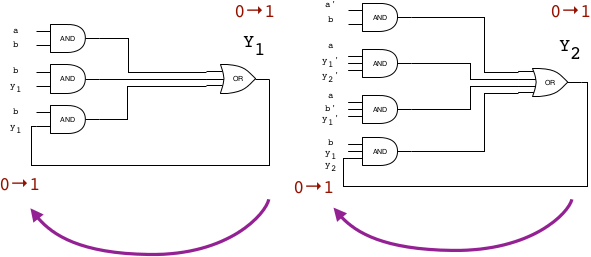
\includegraphics[width=.8\textwidth]{ch7/image30}
\end{figure}
Dans la boucle de rétroaction, la valeur de chacune des deux variables ($Y_1$ et $Y_2$) passe de $0$ à $1$. Or la transition dit $00\rightarrow 11$ donc le changement de valeur de chacune doit s'effectuer exactement en \emph{même temps} ! Si ces valeurs ne changent pas au même moment (fils de rétroaction de longueur différentes par exemple), il y a deux cas :
\begin{itemize}
	\item $Y_1$ a été plus vite que $Y_2$ ($Y_1Y_2=10$)
	\item $Y_2$ a été plus vite que $Y_1$ ($Y_1Y_2=01$)
\end{itemize} 
Donc au lieu de faire $00\rightarrow 11$ on fera $00\rightarrow 01\rightarrow ?$ ou  $00\rightarrow 10\rightarrow ?$. \emph{Le système présente un comportement non voulu (non-déterministe)}\dots
\begin{figure}[H]
	\centering
	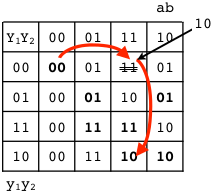
\includegraphics[width=.3\textwidth]{ch7/image31}
\end{figure}
Ainsi, les courses critiques se présenterons lorsque la distance de Hamming entre 2 états codées sera $>1$.
\subsection{Courses critiques et circuits logiques}
Il y a deux approches de résolutions des courses critiques :
\begin{itemize}
	\item on résout en les éliminant $\Rightarrow$ \emph{circuits asynchrones}
	\item on résout en synchronisant afin de mettre à jour le «futur» et ainsi attendre les variables d'états les plus lentes $\Rightarrow$ \emph{circuits synchrones} 
\end{itemize}

\paragraph{Remarque :} 
\begin{itemize}
	\item Ne pas confondre variables d'états et d'entrées
	\item Le changement des variables d'états n'a rien à voir avec le changement des entrées (les entrées sont des variables aléatoires)
	\item On considère que le changement simultané des variables d'entrées est possible
	\item On spécifie dans le cahier des charges le comportement du système dans le cas des variations simultanées des entrées
	\item Parfois, les variations simultanées sont impossibles (réservoir par exemple)
\end{itemize}
\begin{figure}[H]
	\centering
	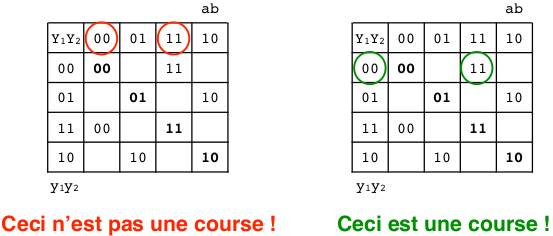
\includegraphics[width=.7\textwidth]{ch7/image32}
\end{figure}
\subsection{Méthodes de résolution des courses critiques pour des circuits asynchrones}
Il existe 3 méthodes, chacune devant être employée si la précédente n'a pas fonctionné (sauf la 1\up{ère} bien évidement), donc \emph{Méthode 1 $\rightarrow$ Méthode 2 $\rightarrow$ Méthode 3}\\
\danger On résout les courses (c-à-d en utilisant ces méthodes) uniquement pour le cas des systèmes asynchrones
\subsubsection{Méthode 1 : codage des états}
Cette méthode consiste à choisir un codage des états tels qu'il n'y ait pas de courses critiques (vu que le codage est arbitraire). Pour ce faire, on dessine un \emph{graphe de codage des états}, permettant de trouver le bon codage ou prouver qu'il n'en existe pas.
\paragraph{Graphe de codage des états :} un carré dont chaque sommet est un état stable, on représente les transitions (états futurs possibles pour chaque état) par un arc orienté. On attribue des codes et on réarrange de manière à ne plus avoir de courses critiques (distance d'Hamming de 1, arcs orientés formeront les arrêtes du carré). 
\begin{figure}[H]
	\centering
	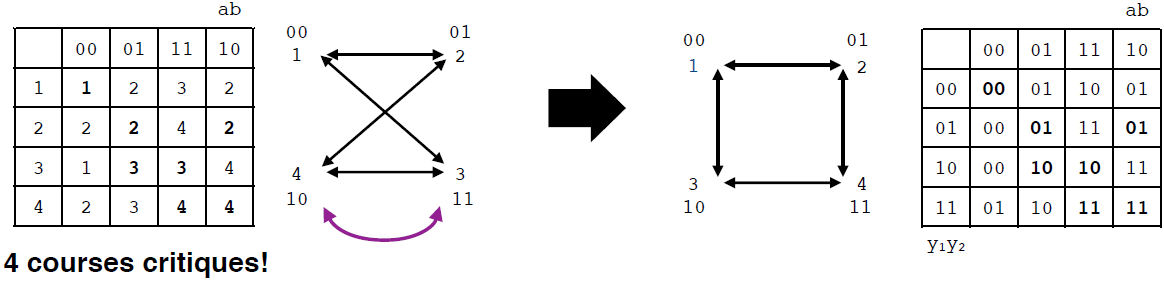
\includegraphics[width=\textwidth]{ch7/image33}
\end{figure}
Il faut néanmoins faire gaffe a switcher les lignes de tel manière a obtenir une K-map !
\begin{figure}[H]
	\centering
	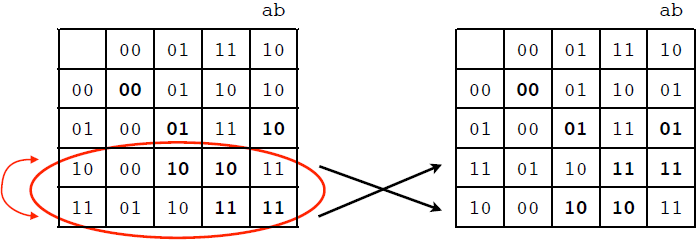
\includegraphics[width=.7\textwidth]{ch7/image34}
\end{figure}
On remarquera qu'il existe plusieurs combinaisons pour le codage des états, influençant la complexité du circuit (mais on ne doit pas en tenir compte :) ).\\
Il n'existe pas toujours une combinaison résolvant les courses critiques $\Rightarrow$ méthode 2
\begin{figure}[H]
	\centering
	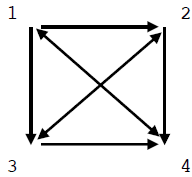
\includegraphics[width=.2\textwidth]{ch7/image35}
\end{figure}
\subsubsection{Méthode 2 : transitions}
On peut transformé une transition pour éviter la course critique (seul le point d'arrivé compte).
\begin{itemize}
	\item Utiliser les \textit{don't cares} :
	\begin{itemize}
		\item on transforme un \textit{don't care} en une transition pour éviter la course critique (par ex. $\textbf{1}\rightarrow 2\rightarrow 3\rightarrow \textbf{3}$)
	\end{itemize}
	\begin{figure}[H]
		\centering
		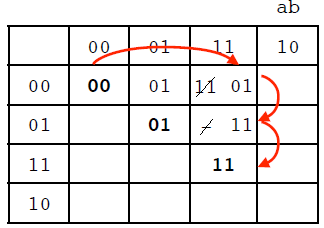
\includegraphics[width=.3\textwidth]{ch7/image36}
	\end{figure}
	\item Modifier les transitions :
	\begin{itemize}
		\item on utilise une transition déjà existante en passant par un autre état (par ex. $\textbf{1}\rightarrow 4\rightarrow 3\rightarrow \textbf{3}$)
	\end{itemize}
	\begin{figure}[H]
		\centering
		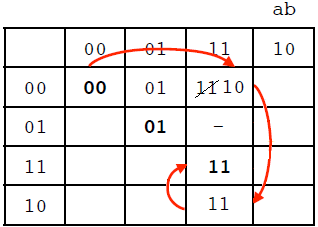
\includegraphics[width=.3\textwidth]{ch7/image37}
	\end{figure}
\end{itemize}
Les 2 sont bons !\\
Si ce n'est pas possible $\Rightarrow$ méthode 3
\subsubsection{Méthode 3 : état supplémentaire}
\textbf{Si et uniquement si} les 2 méthodes précédentes ont échouées, on rajoute une variable d'états (plutôt couteux me direz-vous\dots) et on utilise ces nouveaux états comme intermédiaire de transition afin de résoudre les problèmes de courses.\\
Remarquons que toute course qui peut être résolue par les méthodes 1 et 2 avant, doit l'être.
\subsubsection{fautes graves}
\begin{enumerate}
	\item Laisser une course critique alors qu'on demande de faire la synthèse d'un circuit asynchrone.
	\item Ne pas appliquer les méthodes dans le bon ordre.
	\item dériver une K-map qui n'en est pas une (distance de Hamming $>1$ entre les lignes et les colonnes adjacentes).
\end{enumerate}